% !TeX program = xelatex
\documentclass[a4paper,10pt]{article}

% ============================================================================
% សន្លឹកកិច្ចការសិស្ស ស-ខ្មៅ (Student Guided-Inquiry Worksheet - Grade 8 15.4 CIRC4)
% បរិបទ៖ គ្មានស្លាយ LCD — សិស្សប្រើបន្ទាត់កែង (អេគែរ) វាស់លើរូបខ្នាតពិត 1:1 និងវិនិច្ឆ័យកំហុស
% វិធីសាស្ត្រ៖ Van Hiele Symmetry Inquiry + Erroneous-Example Diagnostic Worksheet
% ============================================================================
\usepackage[a4paper, left=1.0cm, right=1.0cm, top=0.80cm, bottom=1.00cm, footskip=0.50cm]{geometry}
\usepackage{amsmath, amssymb}
\usepackage{unicode-math}
\usepackage{fontspec}
\usepackage{array, colortbl}
\usepackage[table]{xcolor}
\usepackage{enumitem}
\usepackage{pifont}
\usepackage{fancyhdr}
\usepackage{lastpage}
\usepackage{tikz}
\usepackage[most]{tcolorbox}
\usetikzlibrary{calc, arrows.meta, angles, quotes, decorations.markings, positioning, babel}

\makeatletter
\let\@expl@@@mark@update@singlecol@structures@@\relax
\makeatother

\providecommand{\NGSFindFonts}{%
  \IfFileExists{C:/Windows/Fonts/cambria.ttc}{%
    \def\NGSSysPath{C:/Windows/Fonts/}%
    \def\NGSUserPath{C:/Users/KIT/AppData/Local/Microsoft/Windows/Fonts/}%
  }{%
    \IfFileExists{./fonts/KhmerOSsiemreap.ttf}{\def\NGSSysPath{./fonts/}\def\NGSUserPath{./fonts/}}{%
    \IfFileExists{../fonts/KhmerOSsiemreap.ttf}{\def\NGSSysPath{../fonts/}\def\NGSUserPath{../fonts/}}{%
    \IfFileExists{../../fonts/KhmerOSsiemreap.ttf}{\def\NGSSysPath{../../fonts/}\def\NGSUserPath{../../fonts/}}{%
    \IfFileExists{../../../fonts/KhmerOSsiemreap.ttf}{\def\NGSSysPath{../../../fonts/}\def\NGSUserPath{../../../fonts/}}{%
    \IfFileExists{../../../../fonts/KhmerOSsiemreap.ttf}{\def\NGSSysPath{../../../../fonts/}\def\NGSUserPath{../../../../fonts/}}{%
    \IfFileExists{../../../../../fonts/KhmerOSsiemreap.ttf}{\def\NGSSysPath{../../../../../fonts/}\def\NGSUserPath{../../../../../fonts/}}{%
    \IfFileExists{../../../../../../fonts/KhmerOSsiemreap.ttf}{\def\NGSSysPath{../../../../../../fonts/}\def\NGSUserPath{../../../../../../fonts/}}{%
      \def\NGSSysPath{../../../../../../../fonts/}\def\NGSUserPath{../../../../../../../fonts/}%
    }}}}}}}%
  }%
}
\NGSFindFonts

\setmathfont[Path={\NGSSysPath}, FontIndex=1, Scale=1.02]{cambria.ttc}
\defaultfontfeatures{Ligatures=TeX}

\setmainfont[
  Path={\NGSUserPath}, Extension=.ttf, Script=Khmer,
  BoldFont={KhmerOSsiemreap}, BoldFeatures={FakeBold=1.8},
  ItalicFont={KhmerOSsiemreap}, ItalicFeatures={FakeSlant=0.25},
  BoldItalicFont={KhmerOSsiemreap}, BoldItalicFeatures={FakeBold=1.8, FakeSlant=0.25}
]{KhmerOSsiemreap}

\newfontfamily\muol[Path={\NGSUserPath}, Extension=.ttf, Script=Khmer]{KhmerOSmuollight}
\newfontfamily\TimesEn[Path={\NGSSysPath}, Extension=.ttf, BoldFont={timesbd}, ItalicFont={timesi}, BoldItalicFont={timesbi}]{times}
\newfontfamily\CalibriFont[Path={\NGSSysPath}, Extension=.ttf]{calibri}

\XeTeXlinebreaklocale "km"
\XeTeXlinebreakskip = 0pt plus 1pt minus 0.1pt

\definecolor{panelgray}{gray}{0.93}
\definecolor{headgray}{gray}{0.85}

\pagestyle{fancy}
\fancyhf{}
\renewcommand{\headrulewidth}{0pt}
\fancyfoot[L]{\fontsize{8.0pt}{10pt}\selectfont អនុវិទ្យាល័យព្រះក្រសាំង \en{|} គណិតវិទ្យា ថ្នាក់ទី៨ \en{---} មេរៀនទី១៥ (២.៣ លក្ខណៈឆ្លុះនៃរង្វង់) \en{|} គ្រូបង្រៀន៖ ហុក ប៊ុនថែន}
\fancyfoot[R]{\fontsize{8.2pt}{10pt}\selectfont ទំព័រ \en{\thepage\ / \pageref{LastPage}}}

\setlength{\parindent}{0pt}
\setlength{\parskip}{0pt}
\setlength{\tabcolsep}{4pt}

\newcommand{\en}[1]{{\TimesEn #1}}
\newcommand{\enbf}[1]{{\TimesEn\bfseries #1}}
\newcommand{\unit}[1]{\,\text{\en{#1}}}
\newcommand{\cnum}[1]{\mbox{\fontsize{10pt}{12pt}\selectfont\ding{\numexpr181+#1\relax}}}
\newcommand{\chkbox}{\tikz[baseline=-0.15ex]\draw[black, line width=0.85pt] (0,0) rectangle (0.24cm,0.24cm);}
\newcommand{\tri}[1]{\ensuremath{\triangle #1}}
\newcommand{\ang}[1]{\ensuremath{\angle #1}}
\newcommand{\arc}[1]{\ensuremath{\overset{\tikz[baseline=-0.55ex]\draw[black, line width=0.55pt] (0,0) to[bend left=40] (1.8ex,0);}{#1}}}
\newcommand{\blank}[1]{\underline{\hspace{#1}}}
\newcommand{\rightbox}[4][0.18]{%
  \draw[black, line width=0.75pt]
    ($(#3)!#1!(#2)$) -- ($($(#3)!#1!(#2)$)+($(#3)!#1!(#4)$)-(#3)$) -- ($(#3)!#1!(#4)$);
}

\newcommand{\secbox}[2]{%
  \begin{tcolorbox}[
    enhanced, sharp corners, colback=headgray, colframe=black,
    boxrule=0.95pt, boxsep=1pt, top=2.5pt, bottom=2.5pt, left=6pt, right=6pt,
    before skip=4.5pt, after skip=3.5pt
  ]
    {\muol\fontsize{9.4pt}{13.5pt}\selectfont #1}\hfill{\fontsize{8.4pt}{11.5pt}\selectfont\textbf{#2}}
  \end{tcolorbox}%
}

\newcolumntype{L}[1]{>{\raggedright\arraybackslash}p{#1}}
\newcolumntype{C}[1]{>{\centering\arraybackslash}p{#1}}

\begin{document}
\fontsize{9.4pt}{14.2pt}\selectfont

% ============================================================================
% ទំព័រទី ១ ៖ ក្បាលសន្លឹកកិច្ចការ + ផ្នែក ក (E2 Van Hiele + Erroneous Example) + ផ្នែក ខ (E3 ជាទូទៅ + គំរូទី១)
% ============================================================================
\begin{tcolorbox}[
  enhanced, sharp corners, colback=white, colframe=black,
  boxrule=1.1pt, boxsep=2.5pt, top=3.5pt, bottom=3.5pt, left=6pt, right=6pt, after skip=4pt
]
  \begin{minipage}[c]{12.2cm}
    {\muol\fontsize{10.6pt}{15pt}\selectfont សន្លឹកកិច្ចការសិស្ស ១៥.៤ ៖ លក្ខណៈឆ្លុះនៃរង្វង់ និងលំហាត់សំយោគ}\\[3pt]
    ឈ្មោះសិស្ស៖ \blank{4.2cm}\quad ក្រុមទី៖ \blank{1.1cm}\quad ថ្នាក់ទី៨៖ \blank{1.2cm}\\[3pt]
    \textbf{បេសកកម្មបុរាណវិទូ \en{E1}៖} តើរកផ្ចិត $O$ នៃបំណែកធ្នូចានបុរាណដោយប្រើអេគែរតាមវិធីណា? \blank{3.4cm}
  \end{minipage}\hfill%
  \begin{minipage}[c]{5.8cm}
    \centering
    {\fontsize{7.6pt}{9.5pt}\selectfont\textbf{បន្ទះផ្ទៀងខ្នាតពិត \en{5.00 cm (Actual Size 100\%)}}}\\[1.5pt]
    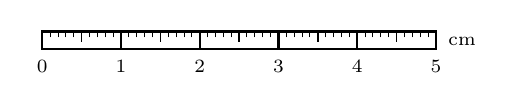
\begin{tikzpicture}[x=1cm, y=1cm]
      \draw[black, line width=0.9pt] (0,0) rectangle (5.0,0.22);
      \foreach \x in {0,1,2,3,4,5} {
        \draw[black, line width=0.8pt] (\x,0) -- (\x,0.22);
        \node[below=0.5pt, font=\fontsize{6.8pt}{8pt}\selectfont] at (\x,0) {\en{\x}};
      }
      \foreach \x in {0.5,1.5,2.5,3.5,4.5} {
        \draw[black, line width=0.6pt] (\x,0.09) -- (\x,0.22);
      }
      \foreach \x in {0.1,0.2,0.3,0.4,0.6,0.7,0.8,0.9,1.1,1.2,1.3,1.4,1.6,1.7,1.8,1.9,2.1,2.2,2.3,2.4,2.6,2.7,2.8,2.9,3.1,3.2,3.3,3.4,3.6,3.7,3.8,3.9,4.1,4.2,4.3,4.4,4.6,4.7,4.8,4.9} {
        \draw[black, line width=0.35pt] (\x,0.15) -- (\x,0.22);
      }
      \node[right=1pt, font=\fontsize{6.8pt}{8pt}\selectfont] at (5.0,0.10) {\en{cm}};
    \end{tikzpicture}
  \end{minipage}
\end{tcolorbox}

% -------------------- ផ្នែក ក (E2 Explore - Van Hiele + Erroneous Example) --------------------
\secbox{ផ្នែក ក \enbf{(E2 Explore)} ៖ រុករកលក្ខណៈឆ្លុះ \enbf{1:1} និងវិនិច្ឆ័យសម្រាយបញ្ជាក់ខុស}{១១ នាទី \en{---} ប្រើបន្ទាត់កែង (អេគែរ) និងបន្ទាត់ក្រិត}

\begin{minipage}[t]{7.2cm}
  \vspace{0pt}
  \begin{tcolorbox}[
    enhanced, sharp corners, colback=white, colframe=black,
    boxrule=0.8pt, boxsep=1.5pt, top=3pt, bottom=3pt, left=2pt, right=2pt
  ]
    \centering
    {\fontsize{8.2pt}{10.5pt}\selectfont\textbf{រង្វង់ខ្នាតពិត \en{1:1} ៖ $C(O, 2.00\unit{cm})$, $AB\perp CD$}}\\[2pt]
    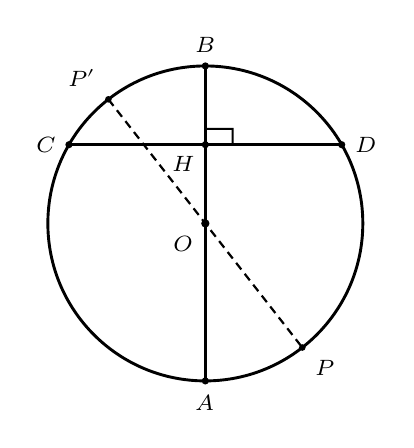
\begin{tikzpicture}[x=1cm, y=1cm, every node/.style={font=\footnotesize, text=black}]
      \coordinate (O) at (0,0);
      \pgfmathsetmacro{\R}{2.00}
      % Vertical diameter AB: A bottom (-90), B top (90)
      \coordinate (A) at (0,-\R);
      \coordinate (B) at (0,\R);
      % Horizontal chord CD at y = 1.00 cm -> half-chord HC = HD = sqrt(4 - 1) = 1.732 cm!
      \pgfmathsetmacro{\xh}{sqrt(\R*\R - 1.00*1.00)}
      \coordinate (C) at (-\xh,1.00);
      \coordinate (D) at (\xh,1.00);
      \coordinate (H) at (0,1.00);
      % Point symmetry P' opposite P at -52 / 128 degrees (cleanly separated from C at 150 and B at 90)
      \coordinate (P) at (-52:\R);
      \coordinate (Pp) at (128:\R);

      \draw[black, line width=1.05pt] (O) circle (\R);
      \draw[black, line width=1.15pt] (A) -- (B);
      \draw[black, line width=1.05pt] (C) -- (D);
      \draw[black, line width=0.8pt, densely dashed] (Pp) -- (P);
      \rightbox[0.20]{B}{H}{D}

      \fill[black] (O) circle (1.5pt) node[below left=1.5pt] {$O$};
      \fill[black] (A) circle (1.3pt) node[below=1.5pt] {$A$};
      \fill[black] (B) circle (1.3pt) node[above=1.5pt] {$B$};
      \fill[black] (C) circle (1.3pt) node[left=1.5pt] {$C$};
      \fill[black] (D) circle (1.3pt) node[right=1.5pt] {$D$};
      \fill[black] (H) circle (1.3pt) node[below left=1pt] {$H$};
      \fill[black] (P) circle (1.2pt) node[below right=1.5pt] {$P$};
      \fill[black] (Pp) circle (1.2pt) node[above left=1.5pt] {$P'$};
    \end{tikzpicture}
  \end{tcolorbox}
\end{minipage}\hfill%
\begin{minipage}[t]{11.4cm}
  \vspace{0pt}
  \textbf{១. ពិសោធន៍វាស់ផ្ទៀងលក្ខណៈឆ្លុះលើរង្វង់ខ្នាតពិតខាងឆ្វេង ($r = 2.00\unit{cm}$)៖}\\[2.5pt]
  $\bullet$ \textbf{ផ្ចិតឆ្លុះ $O$ (ឧទាហរណ៍ទី១)៖} អង្កត់ផ្ចិត $PP'$ កាត់តាម $O$ មាន៖\\
  \hspace*{0.3cm}$OP = \blank{1.3cm}\unit{cm}$ និង $OP' = \blank{1.3cm}\unit{cm} \Rightarrow P$ និង $P'$ ឆ្លុះគ្នាធៀបនឹង \blank{1.0cm} ។\\[2.5pt]
  $\bullet$ \textbf{អ័ក្សឆ្លុះ $AB$ (ឧទាហរណ៍ទី២--៣)៖} អង្កត់ផ្ចិត $AB \perp$ អង្កត់ធ្នូ $CD$ ត្រង់ $H$៖\\
  \hspace*{0.3cm}វាស់ប្រវែង៖ $HC \approx \blank{1.3cm}\unit{cm}$ និង $HD \approx \blank{1.3cm}\unit{cm} \Rightarrow H$ ជា \blank{2.2cm} នៃ $CD$ ។\\
  \hspace*{0.3cm}បើបត់រង្វង់តាមអង្កត់ផ្ចិត $AB$ នោះធ្នូ $\arc{CB}$ ត្រួតស៊ីគ្នាលើធ្នូ \blank{1.2cm} ។\\[4pt]
  \begin{tcolorbox}[
    enhanced, sharp corners, colback=panelgray, colframe=black,
    boxrule=0.85pt, boxsep=2pt, top=3pt, bottom=3pt, left=5pt, right=5pt
  ]
    \begin{minipage}[c]{7.8cm}
      \textbf{២. វិនិច្ឆ័យសម្រាយបញ្ជាក់ខុសរបស់សិស្ស «តារា»៖}\\
      {\fontsize{8.7pt}{12.8pt}\selectfont
      តារាអះអាងថា៖ \textit{«ក្នុងរូបស្ដាំ អង្កត់ផ្ចិត $AB$ កាត់តាមចំណុចកណ្ដាល $O$ នៃអង្កត់ធ្នូ $EF$ ដូចនេះតាមទ្រឹស្ដីបទ គេទាញបាន $AB \perp EF$ ជានិច្ច!»}\\[2.5pt]
      $\bullet$ តើអំណះអំណាងរបស់តារាត្រូវឬខុស? \chkbox\ ត្រូវ \quad \chkbox\ ខុស\\[2pt]
      $\bullet$ ហេតុអ្វី? ព្រោះអង្កត់ធ្នូ $EF$ ខ្លួនវាជា \blank{2.8cm}\\
      $\bullet$ លក្ខខណ្ឌដែលតារាភ្លេច៖ អង្កត់ធ្នូនោះត្រូវតែ \textbf{មិនមែនជា} \blank{2.0cm} !}
    \end{minipage}\hfill%
    \begin{minipage}[c]{2.9cm}
      \centering
      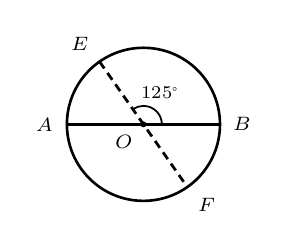
\begin{tikzpicture}[scale=0.90, every node/.style={font=\scriptsize, text=black}]
        \coordinate (O) at (0,0);
        \pgfmathsetmacro{\R}{1.08}
        \draw[black, line width=0.95pt] (O) circle (\R);
        \draw[black, line width=1.0pt] (-\R,0) node[left=1pt]{$A$} -- (\R,0) node[right=1pt]{$B$};
        \draw[black, line width=1.0pt, densely dashed] (125:\R) node[above left=0.5pt]{$E$} -- (-55:\R) node[below right=0.5pt]{$F$};
        \draw[black, line width=0.65pt] (0.26,0) arc (0:125:0.26);
        \node[font=\fontsize{6.5pt}{8pt}\selectfont] at (62:0.50) {$125^\circ$};
        \fill[black] (O) circle (1.2pt) node[below left=0.5pt]{$O$};
      \end{tikzpicture}
    \end{minipage}
  \end{tcolorbox}
\end{minipage}

% -------------------- ផ្នែក ខ (E3 Explain + គំរូទី១) --------------------
\secbox{ផ្នែក ខ \enbf{(E3 Explain)} ៖ សង្ខេបប្រអប់ «ជាទូទៅ» (ទំ.២០២) និងលំហាត់គំរូទី១ (ទំ.២០៣)}{៦ នាទី \en{---} បំពេញប្រអប់ទ្រឹស្ដីបទ និងសម្រាយបញ្ជាក់តាមអ័ក្សឆ្លុះ}

\begin{minipage}[t]{10.3cm}
  \vspace{2pt}
  \textbf{១. ជាទូទៅ (សៀវភៅគោល ទំ.២០២)៖}\\[3pt]
  $\bullet$ រង្វង់មាន\textbf{ផ្ចិតឆ្លុះ}តែមួយគត់គឺ \blank{2.4cm} របស់វា ។\\[3pt]
  $\bullet$ គ្រប់ \blank{2.6cm} ទាំងអស់ ជា\textbf{អ័ក្សឆ្លុះ}នៃរង្វង់ ។\\[3pt]
  $\bullet$ អង្កត់ផ្ចិតដែលកាត់តាមចំណុចកណ្ដាលនៃអង្កត់ធ្នូ (\textbf{មិនមែនជា} \blank{2.1cm}) \blank{1.7cm} នឹងអង្កត់ធ្នូនោះ ហើយចែកធ្នូស្កាត់ជាពីរផ្នែក \blank{1.7cm} ។\\[3pt]
  $\bullet$ អង្កត់ផ្ចិតដែលកែងនឹងអង្កត់ធ្នូមួយ ត្រូវចែក \blank{1.9cm} និង \blank{1.5cm} ជាពីរផ្នែកប៉ុនគ្នា ។\\[3pt]
  $\bullet$ \textbf{វិបាកអង្កត់ធ្នូស្របគ្នា (ទំ.២០៣)៖} បើ $AB \parallel CD$ នោះធ្នូចន្លោះ $\arc{AC} = \blank{1.4cm}$ ។
\end{minipage}\hfill%
\begin{minipage}[t]{8.3cm}
  \vspace{0pt}
  \begin{tcolorbox}[
    enhanced, sharp corners, colback=panelgray, colframe=black,
    boxrule=0.85pt, boxsep=2pt, top=3pt, bottom=3pt, left=5pt, right=5pt
  ]
    {\muol\fontsize{8.8pt}{12.5pt}\selectfont ធនាគារហេតុផល \enbf{(Warrant Bank)} សម្រាប់យោង៖}\\[3pt]
    {\fontsize{8.6pt}{13.2pt}\selectfont
    \cnum{1} \textbf{ផ្ចិតនិងអ័ក្សឆ្លុះ៖} $O$ ជាផ្ចិតឆ្លុះ; គ្រប់អង្កត់ផ្ចិតជាអ័ក្សឆ្លុះ\\
    \cnum{2} \textbf{អង្កត់ផ្ចិត $\perp$ អង្កត់ធ្នូ៖} ចែកអង្កត់ធ្នូ និងធ្នូជាពីរផ្នែកប៉ុនគ្នា\\
    \cnum{3} \textbf{អង្កត់ផ្ចិតកាត់កណ្ដាលអង្កត់ធ្នូ ($\ne$ អង្កត់ផ្ចិត)៖} កែងនឹងអង្កត់ធ្នូ\\
    \cnum{4} \textbf{អង្កត់ធ្នូស្របគ្នា៖} $AB \parallel CD \Rightarrow \arc{AC} = \arc{BD}$\\
    \cnum{5} \textbf{ចម្ងាយពីផ្ចិតស្មើគ្នា៖} $OQ\perp AB, OR\perp CD, OQ=OR \iff AB=CD$}
  \end{tcolorbox}
\end{minipage}

\vspace{4pt}
\begin{tcolorbox}[
  enhanced, sharp corners, colback=white, colframe=black,
  boxrule=0.85pt, boxsep=2pt, top=3pt, bottom=3pt, left=6pt, right=6pt
]
  \textbf{២. លំហាត់គំរូទី១ (ទំ.២០៣ — ស្រាយបញ្ជាក់តាមការបត់រូបធៀបនឹងអ័ក្សឆ្លុះ)៖} គេមានអង្កត់ផ្ចិត $AB \perp$ អង្កត់ធ្នូ $CD$ ត្រង់ $H$ (មើលរូបខ្នាតពិតខាងលើ) ។\\[2.5pt]
  $\bullet$ បើគេបត់រូបតាមបន្ទាត់ $AB$ ដែលជា \blank{2.2cm} នៃរង្វង់ នោះចំណុច $C$ ត្រួតស៊ីគ្នាលើចំណុច \blank{1.0cm} ។\\[2.5pt]
  $\bullet$ នាំឱ្យប្រវែង $HC = \blank{1.3cm}$ ហើយធ្នូស្កាត់ $\arc{CB} = \blank{1.3cm}$ និង $\arc{CA} = \blank{1.3cm}$ ។
\end{tcolorbox}

\newpage
% ============================================================================
% ទំព័រទី ២ ៖ ផ្នែក គ (E4 គំរូទី២ + ប្រតិបត្តិទំ.២០៣) + ផ្នែក ឃ (E5 លំហាត់ទី៤ + ពីតាករ) + ផ្នែក ង (Exit & HW)
% ============================================================================
\secbox{ផ្នែក គ \enbf{(E4 Elaborate)} ៖ អង្កត់ធ្នូស្របគ្នា — លំហាត់គំរូទី២ និងប្រតិបត្តិ (ទំ.២០៣)}{១០ នាទី \en{---} គូសបន្ទាត់ជំនួយ និងបំពេញជំហាន}

\begin{minipage}[t]{9.25cm}
  \begin{tcolorbox}[
    enhanced, sharp corners, colback=white, colframe=black,
    boxrule=0.8pt, boxsep=2pt, top=3pt, bottom=3pt, left=5pt, right=5pt
  ]
    \textbf{លំហាត់គំរូទី២ (ទំ.២០៣)៖} ស្រាយបញ្ជាក់ថា ធ្នូពីរនៅចន្លោះអង្កត់ធ្នូពីរស្របគ្នា ($AB \parallel CD$) ជាធ្នូប៉ុនគ្នា ($\arc{AC}=\arc{BD}$) ៖\\[3pt]
    \begin{minipage}[c]{3.15cm}
      \centering
      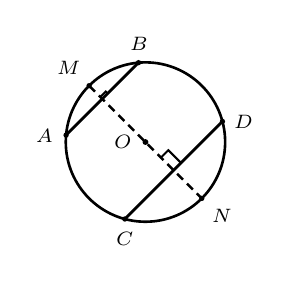
\begin{tikzpicture}[scale=0.88, every node/.style={font=\scriptsize, text=black}]
        \coordinate (O) at (0,0);
        \pgfmathsetmacro{\R}{1.15}
        \coordinate (M) at (135:\R);
        \coordinate (N) at (-45:\R);
        \coordinate (A) at (175:\R);
        \coordinate (B) at (95:\R);
        \coordinate (C) at (-105:\R);
        \coordinate (D) at (15:\R);
        \coordinate (P) at ($ (A)!0.5!(B) $);
        \coordinate (Q) at ($ (C)!0.5!(D) $);
        \draw[black, line width=0.95pt] (O) circle (\R);
        \draw[black, line width=1.0pt] (A) -- (B) (C) -- (D);
        \draw[black, line width=0.85pt, densely dashed] (M) -- (N);
        \rightbox[0.15]{M}{P}{B}
        \rightbox[0.15]{M}{Q}{D}
        \fill[black] (O) circle (1.2pt) node[left=1.5pt] {$O$};
        \fill[black] (M) circle (1.1pt) node[above left=0.5pt] {$M$};
        \fill[black] (N) circle (1.1pt) node[below right=0.5pt] {$N$};
        \fill[black] (A) circle (1.1pt) node[left=1pt] {$A$};
        \fill[black] (B) circle (1.1pt) node[above=1pt] {$B$};
        \fill[black] (C) circle (1.1pt) node[below=1pt] {$C$};
        \fill[black] (D) circle (1.1pt) node[right=1pt] {$D$};
      \end{tikzpicture}
    \end{minipage}\hfill%
    \begin{minipage}[c]{5.60cm}
      {\fontsize{8.7pt}{13.2pt}\selectfont
      $\bullet$ គូសអង្កត់ផ្ចិតជំនួយ $MN \perp AB$ ត្រង់ $P$ ។\\
      $\bullet$ ដោយ $AB \parallel CD \Rightarrow MN \;\blank{0.6cm}\; CD$ ត្រង់ $Q$ ។\\
      $\bullet$ តាម \cnum{1}--\cnum{2}៖ $A$ ឆ្លុះនឹង \blank{0.7cm} ហើយ $C$ ឆ្លុះនឹង \blank{0.7cm} ធៀបនឹងអ័ក្ស $MN$ ។\\
      $\bullet$ ដូចនេះ ធ្នូ $\arc{AC}$ និង $\arc{BD}$ ឆ្លុះគ្នាធៀបនឹង $MN \Rightarrow \arc{AC} = \blank{1.1cm}$ ។}
    \end{minipage}
  \end{tcolorbox}
\end{minipage}\hfill%
\begin{minipage}[t]{9.25cm}
  \begin{tcolorbox}[
    enhanced, sharp corners, colback=white, colframe=black,
    boxrule=0.8pt, boxsep=2pt, top=3pt, bottom=3pt, left=5pt, right=5pt
  ]
    \textbf{ប្រតិបត្តិ (ទំ.២០៣)៖} រង្វង់ផ្ចិត $O$ មានអង្កត់ផ្ចិត $AD$ ហើយ $AB \parallel CD$ ។ ចូរបង្ហាញថា $AB = CD$ ៖\\[3pt]
    \begin{minipage}[c]{3.15cm}
      \centering
      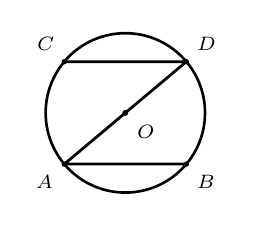
\begin{tikzpicture}[scale=0.88, every node/.style={font=\scriptsize, text=black}]
        \coordinate (O) at (0,0);
        \pgfmathsetmacro{\R}{1.15}
        \coordinate (A) at (-140:\R);
        \coordinate (D) at (40:\R);
        \coordinate (B) at (-40:\R);
        \coordinate (C) at (140:\R);
        \draw[black, line width=0.95pt] (O) circle (\R);
        \draw[black, line width=1.0pt] (A) -- (D) (A) -- (B) (C) -- (D);
        \fill[black] (O) circle (1.2pt) node[below right=1pt] {$O$};
        \fill[black] (A) circle (1.1pt) node[below left=0.5pt] {$A$};
        \fill[black] (B) circle (1.1pt) node[below right=0.5pt] {$B$};
        \fill[black] (C) circle (1.1pt) node[above left=0.5pt] {$C$};
        \fill[black] (D) circle (1.1pt) node[above right=0.5pt] {$D$};
      \end{tikzpicture}
    \end{minipage}\hfill%
    \begin{minipage}[c]{5.60cm}
      {\fontsize{8.7pt}{13.2pt}\selectfont
      $\bullet$ ដោយ $AB \parallel CD$ តាមហេតុផល \cnum{4}៖\\
      \hspace*{0.25cm}$\arc{AC} = \blank{1.2cm}$ ។\\
      $\bullet$ តែ $AD$ ជាអង្កត់ផ្ចិត ($180^\circ$)៖\\
      \hspace*{0.25cm}$\arc{AB} = 180^\circ - \blank{1.0cm}$\\
      \hspace*{0.25cm}$\arc{CD} = 180^\circ - \blank{1.0cm}$\\
      $\bullet$ នាំឱ្យ $\arc{AB} = \arc{CD} \Rightarrow AB = \blank{1.1cm}$ ។}
    \end{minipage}
  \end{tcolorbox}
\end{minipage}

\vspace{3pt}
\textbf{សំណួរត្រិះរិះ (\en{EIA 30s})៖} ក្រៅពីប្រើធ្នូ តើអាចស្រាយបញ្ជាក់ $\tri{OAB} \cong \tri{ODC}$ តាមករណីអ្វី? ចម្លើយ៖ \blank{5.2cm}

% -------------------- ផ្នែក ឃ (E5 Synthesis Exercise #4 p.204 + Pythagoras) --------------------
\secbox{ផ្នែក ឃ \enbf{(E5 Evaluate)} ៖ លំហាត់សំយោគពិជគណិត--ធរណីមាត្រ (លំហាត់ទី៤ ទំ.២០៤ និងពីតាករ)}{៦.៥ នាទី \en{---} ចម្ងាយស្មើគ្នាពីផ្ចិត និងកាំកែងអង្កត់ធ្នូ}

\begin{minipage}[c]{4.9cm}
  \begin{tcolorbox}[
    enhanced, sharp corners, colback=white, colframe=black,
    boxrule=0.8pt, boxsep=1.5pt, top=2.5pt, bottom=2.5pt, left=2pt, right=2pt
  ]
    \centering
    {\fontsize{8.0pt}{10pt}\selectfont\textbf{លំហាត់ទី៤ (ទំ.២០៤)៖ $OQ=OR$}}\\[2pt]
    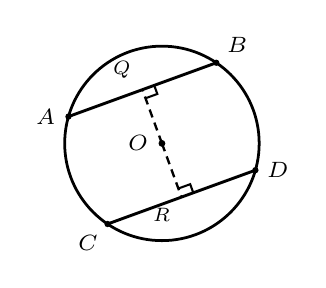
\begin{tikzpicture}[scale=0.95, every node/.style={font=\footnotesize, text=black}]
      \coordinate (O) at (0,0);
      \pgfmathsetmacro{\R}{1.30}
      \coordinate (A) at (164:\R);
      \coordinate (B) at (56:\R);
      \coordinate (C) at (-124:\R);
      \coordinate (D) at (-16:\R);
      \coordinate (Q) at ($ (A)!0.5!(B) $);
      \coordinate (R) at ($ (C)!0.5!(D) $);
      \draw[black, line width=1.0pt] (O) circle (\R);
      \draw[black, line width=1.05pt] (A) -- (B) (C) -- (D);
      \draw[black, line width=0.85pt, densely dashed] (O) -- (Q) (O) -- (R);
      \rightbox[0.16]{O}{Q}{B}
      \rightbox[0.16]{O}{R}{D}
      \fill[black] (O) circle (1.3pt) node[left=1.5pt] {$O$};
      \fill[black] (A) circle (1.2pt) node[left=1pt] {$A$};
      \fill[black] (B) circle (1.2pt) node[above right=0.5pt] {$B$};
      \fill[black] (C) circle (1.2pt) node[below left=0.5pt] {$C$};
      \fill[black] (D) circle (1.2pt) node[right=1pt] {$D$};
      \node[above left=0.8pt, font=\scriptsize] at (Q) {$Q$};
      \node[below left=0.8pt, font=\scriptsize] at (R) {$R$};
    \end{tikzpicture}
  \end{tcolorbox}
\end{minipage}\hfill%
\begin{minipage}[c]{13.7cm}
  \textbf{១. លំហាត់ទី៤ (ទំ.២០៤)៖} គេឱ្យរង្វង់ផ្ចិត $O$ ដែល $OQ\perp AB$, $OR\perp CD$ និង $OQ = OR$ ហើយ $AB = 6x + 14$ និង $CD = -4x + 4$ ។ គណនាប្រវែងអង្កត់ធ្នូ $AB$ និង $CD$ ៖\\[3pt]
  $\bullet$ \textbf{ជំហានទី១ (តាម \cnum{5})៖} ដោយ $OQ\perp AB, OR\perp CD$ និង $OQ=OR \Rightarrow AB = \blank{1.4cm}$ ។\\[3pt]
  $\bullet$ \textbf{ជំហានទី២ (រក $x$)៖} $6x + 14 = \blank{2.2cm} \Rightarrow 10x = \blank{1.6cm} \Rightarrow x = \blank{1.3cm}$ ។\\[3pt]
  $\bullet$ \textbf{ជំហានទី៣ (ផ្ទៀងផ្ទាត់ $>0$)៖} $AB = 6(\blank{0.9cm}) + 14 = \blank{1.3cm}$ និង $CD = \blank{1.3cm}$ ។
\end{minipage}

\vspace{3.5pt}
\begin{tcolorbox}[
  enhanced, sharp corners, colback=panelgray, colframe=black,
  boxrule=0.8pt, boxsep=2pt, top=2.5pt, bottom=2.5pt, left=6pt, right=6pt
]
  \textbf{២. លំហាត់គន្លឹះពីតាករ (ត្រៀមសំណួរ \en{C} និងលំហាត់ទី៩)៖} ក្នុងរង្វង់ $C(O, 13\unit{cm})$ អង្កត់ផ្ចិតកែងនឹងអង្កត់ធ្នូ $AB$ ត្រង់ $M$ ដែលចម្ងាយ $OM = 5\unit{cm}$ ។ គណនា $AM$ និង $AB$ ៖\\[2pt]
  $\bullet$ ក្នុង $\tri{OMA}$ កែងត្រង់ $M$៖ $AM = \sqrt{OA^2 - OM^2} = \sqrt{\blank{1.1cm}^2 - \blank{0.9cm}^2} = \blank{1.2cm}\unit{cm} \Rightarrow$ តាម \cnum{2} បាន $AB = 2 \times AM = \blank{1.3cm}\unit{cm}$ ។
\end{tcolorbox}

% -------------------- ផ្នែក ង (E5 Exit Check & Homework) --------------------
\secbox{ផ្នែក ង \enbf{(E5 Exit Check \& Homework)} ៖ វាយតម្លៃរហ័ស \enbf{A--D} និងកិច្ចការផ្ទះ (ទំ.២០៤)}{៣.៥ នាទី \en{+} កិច្ចការផ្ទះ}

{\renewcommand{\arraystretch}{1.28}
\begin{tabular}{|C{0.7cm}|L{12.8cm}|C{2.4cm}|C{2.2cm}|}
  \hline
  \cellcolor{panelgray}\textbf{កូដ} & \cellcolor{panelgray}\textbf{អំណះអំណាងវិនិច្ឆ័យ (គូស \ding{51} ក្នុងប្រអប់ និងបញ្ជាក់លេខហេតុផល \cnum{1}--\cnum{5})} & \cellcolor{panelgray}\textbf{ជម្រើស} & \cellcolor{panelgray}\textbf{លេខហេតុផល} \\ \hline
  \enbf{A} & រង្វង់មានអ័ក្សឆ្លុះរាប់មិនអស់ (គ្រប់អង្កត់ផ្ចិត) ប៉ុន្តែមានផ្ចិតឆ្លុះតែមួយគត់គឺចំណុចផ្ចិត $O$ ។ & \chkbox\ ត្រូវ \;\; \chkbox\ ខុស & \blank{1.4cm} \\ \hline
  \enbf{B} & បើអង្កត់ផ្ចិត $AB$ កាត់តាមចំណុចកណ្ដាលនៃអង្កត់ធ្នូ $EF$ ណាមួយ នោះ $AB \perp EF$ ជានិច្ចឥតលក្ខខណ្ឌ ។ & \chkbox\ ត្រូវ \;\; \chkbox\ ខុស & \blank{1.4cm} \\ \hline
  \enbf{C} & ក្នុងរង្វង់កាំ $r=13\unit{cm}$ បើចម្ងាយពីផ្ចិតទៅអង្កត់ធ្នូ $AB$ ស្មើ $5\unit{cm}$ នោះប្រវែង $AB = 24\unit{cm}$ ។ & \chkbox\ ត្រូវ \;\; \chkbox\ ខុស & \blank{1.4cm} \\ \hline
  \enbf{D} & ក្នុងរង្វង់តែមួយ បើអង្កត់ធ្នូពីរស្របគ្នា ($AB \parallel CD$) នោះធ្នូស្ថិតនៅចន្លោះវាមានរង្វាស់ប៉ុនគ្នា ។ & \chkbox\ ត្រូវ \;\; \chkbox\ ខុស & \blank{1.4cm} \\ \hline
\end{tabular}}

\vspace{4pt}
\begin{tcolorbox}[
  enhanced, sharp corners, colback=white, colframe=black,
  boxrule=0.9pt, boxsep=2pt, top=3pt, bottom=3pt, left=6pt, right=6pt
]
  \begin{minipage}[c]{12.2cm}
    {\muol\fontsize{9.0pt}{13pt}\selectfont កិច្ចការផ្ទះបញ្ចប់មេរៀនទី១៥} \textbf{(សៀវភៅគោល ទំព័រ ២០៤ ៖ លំហាត់ទី៨, ទី៩ និង ទី១០ក)}\\[2.5pt]
    $\bullet$ \textbf{១. លំហាត់ទី៨ (ទំ.២០៤)៖} កន្លះរង្វង់អង្កត់ផ្ចិត $AB$ និងអង្កត់ធ្នូ $CD$ ។ គូស $AP\perp CD$ និង $BS\perp CD$ (រូបឆ្វេង) ។ ស្រាយបញ្ជាក់ថា $PC = SD$ (\textit{តម្រុយ៖ គូស $OH\perp CD \Rightarrow HC=HD$ និង $HP=HS$}) ។\\[2pt]
    $\bullet$ \textbf{២. លំហាត់ទី៩ (ទំ.២០៤)៖} ចំណុច $P$ ក្នុង $C(O,r)$ (រូបស្ដាំ) ។ ស្រាយថាអង្កត់ធ្នូកាត់តាម $P$ ដែលកែងនឹង $OP$ ខ្លីជាងគេ ។\\[2pt]
    $\bullet$ \textbf{៣. លំហាត់ទី១០ក (ទំ.២០៤ — សិស្សពូកែ)៖} អង្កត់ធ្នូ $AB>CD$ កាត់គ្នាត្រង់ $K$ ក្រៅរង្វង់; $H, P$ ជាចំណុចកណ្ដាលនៃ $AB, CD$ ។ ស្រាយថា ចំណុចកណ្ដាលនៃ $OK$ ស្មើចម្ងាយពី $O, K, P, H$ ។
  \end{minipage}\hfill%
  \begin{minipage}[c]{5.9cm}
    \centering
    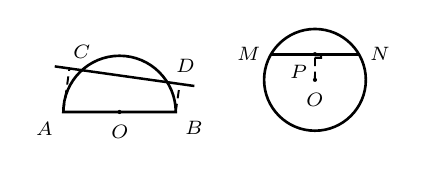
\begin{tikzpicture}[scale=0.68, every node/.style={font=\scriptsize, text=black}]
      \begin{scope}[shift={(0,0)}]
        \coordinate (O) at (1.20,0.45);
        \draw[black, line width=0.95pt] ($(O)+(1.05,0)$) arc (0:180:1.05) -- cycle;
        \coordinate (C) at ($(O)+(132:1.05)$);
        \coordinate (D) at ($(O)+(32:1.05)$);
        \coordinate (A) at ($(O)+(-1.05,0)$);
        \coordinate (B) at ($(O)+(1.05,0)$);
        \coordinate (P) at ($ (C)!(A)!(D) $);
        \coordinate (S) at ($ (C)!(B)!(D) $);
        \draw[black, line width=0.9pt] ($(P)!-0.15!(D)$) -- ($(S)!-0.15!(C)$);
        \draw[black, line width=0.7pt, densely dashed] (A) -- (P) (B) -- (S);
        \fill[black] (O) circle (1.1pt) node[below=1pt]{$O$};
        \node[below left=0pt] at (A) {$A$};
        \node[below right=0pt] at (B) {$B$};
        \node[above=0.5pt] at (C) {$C$};
        \node[above right=0pt] at (D) {$D$};
      \end{scope}
      \begin{scope}[shift={(3.7,0)}]
        \coordinate (O) at (1.15,1.05);
        \draw[black, line width=0.95pt] (O) circle (0.95);
        \coordinate (P) at ($(O)+(0,0.48)$);
        \draw[black, line width=1.0pt] ($(P)+(-0.82,0)$) node[left=0.5pt]{$M$} -- ($(P)+(0.82,0)$) node[right=0.5pt]{$N$};
        \draw[black, line width=0.7pt, densely dashed] (O) -- (P);
        \rightbox[0.14]{O}{P}{$(P)+(0.82,0)$}
        \fill[black] (O) circle (1.1pt) node[below=1pt]{$O$};
        \fill[black] (P) circle (1.1pt) node[below left=0.5pt]{$P$};
      \end{scope}
    \end{tikzpicture}
  \end{minipage}
\end{tcolorbox}

\end{document}
